\documentclass[twocolumn,superscriptaddress]{revtex4-1}
\usepackage{graphicx}
\usepackage{epstopdf}
\usepackage{amsmath}
% \usepackage{hyperref}
\usepackage{booktabs}
\usepackage{color}
\usepackage{multirow}
\setlength{\tabcolsep}{10pt}

\begin{document}

\title{Importance of many-body correlations in glass transition: polydisperse hard spheres as an example} 

\author{Mathieu Leocmach$^a$}
\email{mathieu.leocmach@polytechnique.org}
\altaffiliation[Present address: ]{Laboratoire de Physique, CNRS UMR 5672, Ecole Normale Supérieure de Lyon, 46 allée d'Italie 69364 Lyon cedex 07, France.}
\author{John Russo$^a$}
\email{russoj@iis.u-tokyo.ac.jp}
\author{Hajime Tanaka}
\email{tanaka@iis.u-tokyo.ac.jp}
\affiliation{ {Institute of Industrial Science, University of Tokyo, 4-6-1 Komaba, Meguro-ku, Tokyo 153-8505, Japan} }
\thanks{$^a$M. Leocmach and J. Russo contributed equally to this work.}
\date{Received \today}

\begin{abstract}
Most of the liquid-state theories, including glass-transition theories, are constructed on the basis of two-body density correlations. 
However, we have recently shown that many-body correlations, in particular bond orientational correlations, play a key role in
both the glass transition and the crystallization transition.
Here we show, with numerical simulations of supercooled polydisperse hard spheres systems, that the lengthscale associated with any two-point spatial 
correlation function does not increase toward the glass transition. A growing lengthscale is instead revealed
by considering many-body correlation functions, such as correlators of orientational order,
which follows the lengthscale of the dynamic heterogeneities.
Despite the growing of crystal-like bond orientational order, we reveal that the stability against crystallization with increasing polydispersity
is due to an increasing population of icosahedral arrangements of particles. 
Our results suggest that, for this type of systems, many-body correlations are the link between the vitrification and the crystallization phenomena.
Whether a system is vitrified or crystallized can be controlled by the degree of frustration against crystallization, polydispersity 
in this case.  
\end{abstract}

\maketitle

\section{Introduction}

Amorphous materials have been of prime importance in our technology for millennia, from antique glass works to fashionable phones made of metallic glass. One of the new frontiers of the amorphous technology is in the design of amorphous drugs~\cite{Petit2006,Grzybowska2012}, better absorbed by our metabolism with less side effects, that would be stable at room temperature. The main obstacle is our lack of basic understanding of the physics of the glass transition, without any operative consensus despite half a century of intensive research~\citep{cavagna2009supercooled,BerthierR}.

When cooled below its freezing temperature while avoiding crystallization, a liquid becomes supercooled. Upon further cooling, the dynamics slows down by many orders of magnitude leading to a material that is mechanically a solid without long range positional order, thus called amorphous. It is now known that the dynamics inside a supercooled liquid is heterogeneous, with a length scale that grows when approaching the glass transitionn~\citep{yamamoto1998,Donati1999a} (see~\citep{BerthierR} for a review). The lengthscale defined by the dynamical heterogeneity is not static (one-time spatial correlation) but dynamic (two-time spatial correlation).

The existence of a static (structural) length that would grow and accompany the dynamic heterogeneities is still not clear in the general case. However, in a class of system that includes polydisperse hard spheres, we have shown~\cite{tanaka} that some medium range bond orientational order reminiscent of the crystal exists in the supercooled liquid and grows toward the glass transition in the same way as the dynamical heterogeneity. The presence in glassy materials of structures locally reminiscent of crystals has been confirmed recently in amorphous silicon~\cite{Treacy2012} and in a metallic glass~\cite{Hwang2012}. While bond-orientational order is a member of the class of many-body
correlations between neighbouring particles, it is yet unclear if a similar lengthscale can be extracted
from two-body correlation functions. This question is particularly important considering that the only exact (in the mean-field, infinite dimension approximation) theory of the glass transition, the Mode-coupling theory (MCT), takes as input only two-body quantities. Modern spin-glass-type theories of the structural glass transition~\cite{lubchenko2007,Biroli2008,Parisi2010} are building on the MCT (considered as a mean-field limit), while not taking explicitly into account many-body correlations.


At polydispersities over $6-7\%$, the system need to fractionate to crystallize~\citep{Fasolo2003}. What is the bond order of the reference crystal is then unclear and may challenge our scenario. This is a situation reminiscent of binary hard sphere systems of size ratio close to one~\cite{Hopkins2011b,Hopkins2012} where growing bond order have not been reported~\cite{Charbonneau}. Although it is known that in binary systems locally favored structures play a role in the slowing down of the dynamics~\cite{Coslovich2011,Malins2012}.

In the present study we will use polydisperse hard sphere systems, where we know how to extract meaningful many-body correlations, and look for a two-body quantity that would show the same behavior as the bond order. We will show that the two-body part of the free energy and the two-body part of the structural entropy are unable to capture medium range bond ordered regions or to yield correlation lengths meaningful from the point of view of the glass transition. We thus confirm the medium range crystalline order scenario and test its robustness against increasing polydispersity.
Since bond-orientational order is directly linked to the underlying crystalline structures, we will then address the important question
of what it the mechanism responsible for the avoidance of crystallization. We will show that in the metastable fluid phase crystalline packings
are in competition with icosahedral packings, and that polydispersity acts in favor of the latter ones.

The paper is organized as follows. In Section~\ref{sec:methods} we present the details of the simulations and the order parameters considered in this work. In Section~\ref{sec:results} the results are organized into
a study of the order parameters distribution (Section~\ref{sec:order_parameters}) and their static lengthscales (Section~\ref{sec:lengths}), and a novel method to determine the competition between crystalline structures
and icosahedral packings (Section~\ref{sec:icosahedra}).

\section{Methods}\label{sec:methods}
We run isothermal-isobaric NpT Monte Carlo simulations of $N=4000$ polydisperse hard spheres.
The diameters ($\sigma$) follow a Gaussian distribution $P(\sigma)=\exp{\left[-(\sigma-\sigma_0)^2/2\,s^2\right]}/\sqrt{2\pi} s$,
with polydispersity index $\delta=s/\sigma_0$. In the following we fix the unit of length as $\sigma_0=1$.

Our aim is to compare the behavior of both two-point quantities and many-body quantities with increasing pressure.
Due to the hard-sphere interaction, entropy is the only contribution to the system free energy.
All two-pair correlation quantities are thus derived from the two-body excess entropy~\cite{Nettleton1958,Mountain1971},
defined as
\begin{equation}
s_2=-\frac{\rho}{2}\int dr\left[g(r)\log(g(r))-g(r)+1\right]
\end{equation}

In principle, $s_2$ can be calculated separately for each particle $i$ in the system. In practice, this requires time averages to compute the pair correlation function of each particle, $g_i(r)$. In \cite{tanaka} we averaged on times comparable or longer than the $\alpha$ relaxation, leading to a quantity that was trivially a reflection of the dynamical heterogeneity. 

Here we instead construct an approximate but instantaneous $s_2(i)$ using the pair correlation function $g(r)$
\begin{equation}
s_2(i) = -\frac{\rho}{2}\sum_j \left[g(r_{ij})\log(g(r_{ij}))-g(r_{ij})+1\right].
\end{equation}
This quantity is in very good agreement with the one obtained by calculating the radial distribution function for each
particle, $g_i(r)$, averaged over times comparable to the $\beta$ relaxation time.

More rigorously, one can compute directly the free-energy of each configuration by
measuring the free volume of the particles, defined as the volume ($v(i)$) in which each sphere can freely
move while holding all the other spheres fixed. It has been shown~\cite{Aste2004} that this free
volume is simply related to the pair free-energy ($f_2$) by the following relation
\begin{equation}
f_2=\sum_i f_2(i)=-k_BT\sum_i \log(v(i)/\lambda)
\end{equation}
where $\lambda$ is the thermal wavelength. To compute the free volume we follow previous
studies: first the Voronoi-diagram for each configuration is computed, and the polyhedron
surrounding each particle is determined. The free volume of particle $i$ is then
computed by shifting normally all the faces of the corresponding polyhedron by $\sigma(i)/2$
towards particle $i$, and computing the new volume. This procedure is conducted indipendentely
for each particle and for each configuration.

To study many-body correlations we use the local bond-order analysis introduced by
Steinhardt~\cite{steinhardt}, first applied to study crystal nucleation by
Frenkel and co-workers~\cite{auer}. 
The $\ell$-fold symmetry of a neighbourhood around each particle $i$ is characterised by a $(2\ell+1)$ dimensional complex vector ($\mathbf{q}_l$) as $q_{\ell m}(i)=\frac{1}{N_b(i)}\sum_{j=1}^{N_b(i)} Y_{\ell m}(\mathbf{\hat{r}_{ij}})$, where
$\ell$ is a free integer parameter, and $m$ is an integer
that runs from $m=-\ell$ to $m=\ell$. The functions $Y_{\ell m}$ are the spherical harmonics
and $\mathbf{\hat{r}_{ij}}$ is the vector from particle $i$ to particle $j$.
The sum goes over all neighbouring particles $N_b(i)$ of particle $i$. Usually 
$N_b(i)$ is defined by all particles within a cutoff distance, but in an inhomogeneous system
the cutoff distance would have to change according to the local density. Instead we 
fix $N_b(i)=12$ which is the number of nearest neighbours in icosahedra and close packed crystals (like \textsc{hcp} and \textsc{fcc})
which are known to be the only relevant crystalline structures for hard spheres.

In the analysis, one uses the rotational invariants defined as:
\begin{align}
	q_\ell =& \sqrt{\frac{4\pi}{2l+1} \sum_{m=-\ell}^{\ell} |q_{\ell m}|^2 }, \label{eq:ql}\\
	w_\ell =& \sum_{m_1+m_2+m_3=0} 
			\left( \begin{array}{ccc}
				\ell & \ell & \ell \\
				m_1 & m_2 & m_3 
			\end{array} \right)
			q_{\ell m_1} q_{\ell m_2} q_{\ell m_3}. \label{eq:wl}
\end{align}
where the term in brackets in Eq.~(\ref{eq:wl}) is the Wigner 3-j symbol.
In particular both crystalline and icosahedral neighbourhood have high $q_6$ (strong 6-fold symmetry), with the highest values for the latter. To detect specifically icosahedral order one prefers $w_6$, whose minimum value is obtained only by a perfect icosahedron.

The identification of crystalline particles follows the usual procedure~\cite{auer}. A particle is identified as crystal if
its orientational order is coherent (in symmetry and in orientation) with that of its neighbours.
The scalar product $(\mathbf{q}_6(i)/|\mathbf{q}_6(i)|)\cdot(\mathbf{q}_6(j)/|\mathbf{q}_6(j)|)$ quantifies this similarity. If it exceeds $0.7$ between
two neighbours, they are deemed \emph{connected}. We then identify a particle as crystalline if it is connected with at least $7$ neighbours~\cite{auer}. In a more continuous way, summing the contribution of all the bonds of a given particle, we define the ``crystallinity''~\cite{russo_hs}
\begin{equation}\label{eqn:crystallinity}
 \text{C}(i)=\sum_{j=0}^{N_b(i)}\frac{\mathbf{q}_6(i)\cdot\mathbf{q}_6(j)}{|\mathbf{q}_6(i)|\,|\mathbf{q}_6(j)|}.
\end{equation}

Alternatively, one can coarse-grain $\mathbf{q}_\ell$ over the neighbours~\cite{lechner}
\begin{equation}
	Q_{\ell m}(i) = \frac{1}{N(i)+1}\left( q_{\ell m}(i) +  \sum_{j=0}^{N(i)} q_{\ell m}(j)\right), 
	\label{eq:Qlm}
\end{equation}
to kill locally incoherent orientations (icosahedral order)~\cite{mathieu_icosahedra} and use the resulting invariant $Q_6$ as an indication of crystallinity.

We note that both $\text{C}$ and $Q_6$ are no direct indicator for the presence of crystals, but rather measures for a tendency to promote crystallization.

\section{Results}\label{sec:results}

\begin{figure}
 \centering
 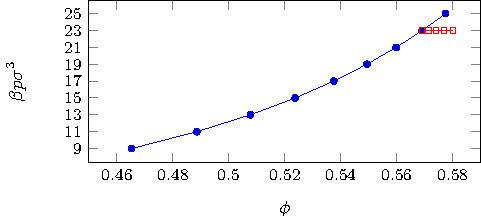
\includegraphics{fig_eos}
 \caption{\textbf{Simulated state points.} The circles (blue curve) represent the equation of state for polydispersity $\delta=7\%$. The squares (red curve) instead are simulation points at the same pressure ($\beta p\sigma^3=23$) but at different polydispersities $\delta$: from low to high volume fraction they correspond to $\delta=7\%,9\%,11\%,13\%,15\%$ respectively.}
 \label{fig:eos}
\end{figure}


Fig.~\ref{fig:eos} shows the equation of state for the simulated state points. In particular
we consider two data-sets. The first one (black circles in the figure) corresponds to
simulations at a constant polydispersity of $\delta=7\%$. For each state point we run $8$ independent
simulation runs and extract configurations for the calculation of correlation lengths.
The second data set (red cicles in the figure) are instead isobaric simulation (at $\beta p\sigma^3=23$)
with increasing polydispersity, $\delta=7\%,9\%,11\%,13\%,15\%$. These state points are used to study
the mechanism by which crystallization is suppressed upon increase of polydispersity, unveiling the
role played by icosahedral arrangement of particles.

\subsection{Order parameter distribution and mobility}\label{sec:order_parameters}

\begin{figure}
	\centering
	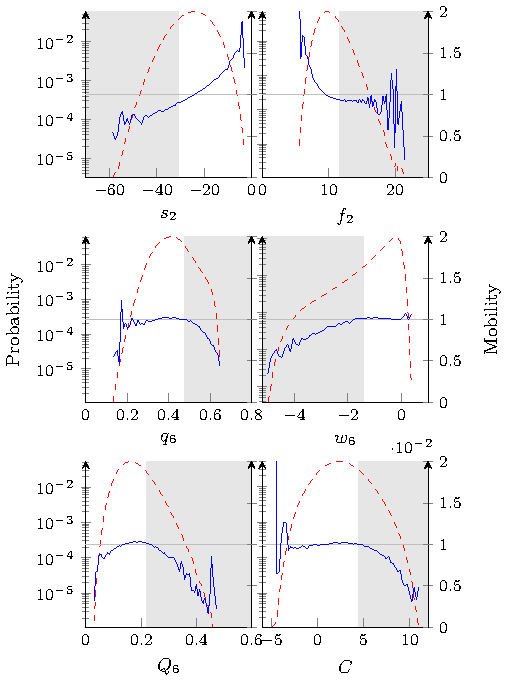
\includegraphics{fig_distrib}
	\caption{\textbf{Probability distribution} (red dash) \textbf{and mobility} (blue continuous) function of various order parameter at $\beta p\sigma^3=25$ and for a time difference corresponding to the $\alpha$-relaxation. Mobility is in unit of mean-square displacement. The limit of the shaded area is at one standard deviation from the mean value of the order parameter in the direction of ordering.}
	\label{fig:distrib}
\end{figure}

We study systematically two-body ($s_2$, $f_2$) and many-body ($q_6$, $w_6$, $Q_6$, $C$) scalar order parameter fields for our highest pressure ($\beta p\sigma^3=25$). Figure~\ref{fig:distrib} shows the probability distribution of these parameters, where the ordered side is depicted as a shaded area. Note that these order parameters are maximazed or
minimazed by different local structures: while \emph{crystalline} order parameters ($Q_6$ and $C$) are maximazed
by local crystalline environments (corresponding to the \textsc{hcp} or \textsc{fcc} crystal), the $w_6$ has its minimum for
icosahedral packings, and $q_6$ grows continously from the fluid phase toward both the crystalline and icosahedral environments.

We first note the absence of any linear coupling between two-body and many-body order parameters.
By plotting the probability distribution function for the metastable fluid on the $f_2$, $Q_6$ and $w_6$ axis, Figure~\ref{fig:f2decoupling} shows the absence of linear correlations between $f_2$ and both $Q_6$ and $w_6$. Since $Q_6$ identifies crystal-like bond-orientationally ordered regions, and $w_6$ locates icosahedral arrangements of particles, it is clear that high $f_2$ regions are not associated with any of these structures. We checked in the same way that $s_2$ is not correlated with many-body parameters.


\begin{figure}
 \centering
 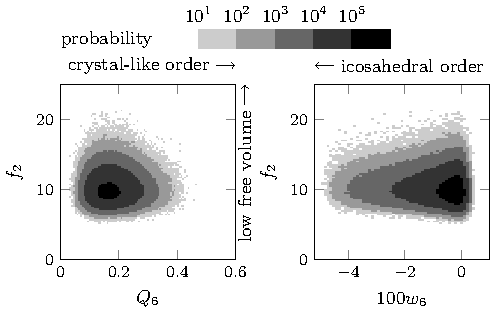
\includegraphics{fig_f2decoupling}
 \caption{\textbf{Correlation between two-body and many-body parameters.} Probability distribution functions in the $f_2$,$Q_6$-map (top) and in the $f_2$,$w_6$-map (bottom) for a metastable fluid with polydispersity $\delta=7\%$ and pressure $\beta p\sigma^3=23$. The parameters are not correlated, even in extreme values.}
 \label{fig:f2decoupling}
\end{figure}

The absence of strong correlations between two-body quantities and both crystalline and icosahedral packings is also evident from
the microscopic dynamics.
To study the correlation between any scalar order parameter $x$ and the displacement of the particles, we define the mobility 
\begin{equation}
	\Delta r^2(x=x_0, t) \equiv \left\langle \frac{
		\sum\limits_i{
			\left\|\mathbf{r}_i(t)-\mathbf{r}_i(0)\right\|^2 \delta(x(i)-x_0)
			}
	}{
		\sum\limits_i{\delta(x(i)-x_0)}
	}\right\rangle,
	\label{eq:mobility}
\end{equation}
shown in Fig.~\ref{fig:distrib} for a time difference corresponding to the $\alpha$-relaxation time. Mobility always decreases with increasing order. The mobilities of bond-order quantities are flat in the disordered regions and decrease when approaching the perfect structure (i.e. icosahedron for $w_6$, crystal cell for $Q_6$ or $C$). By contrast, the mobility of two-body order parameters tends to decrease strongly in the disordered region and less in the ordered region (it is almost flat at high $f_2$). We conclude that many-body quantities describe better the slowing down accompanying good local ordering, while two-body quantities are not clearly correlated to such slower structures.
Note that in Figure~\ref{fig:distrib} both icosahedral packings (low $w_6$ particles) and bond-ordered crystalline regions (high $Q_6$ and $C$) are associated with slow dynamics. As was shown from some of us~\cite{mathieu_icosahedra}, the structures primarily responsible for the slowing down of the dynamics are the crystalline particles, while icosahedral particles act to stop the crystallization process~\cite{russo_hs}.
This will be shown in detail in Section~\ref{sec:icosahedra}.


\subsection{Length-scales}\label{sec:lengths}
\begin{figure}
	\centering
	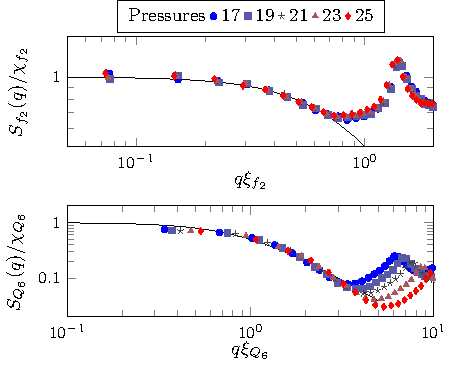
\includegraphics{fig_structurefactor}
	\caption{\textbf{Structure factors} collapse on the Ornstein-Zernike form for (top) $f_2$ and (bottom) $C$. Note how the former are almost similar across pressures.}
	\label{fig:structurefactor}
\end{figure}

\begin{figure}
	\centering
	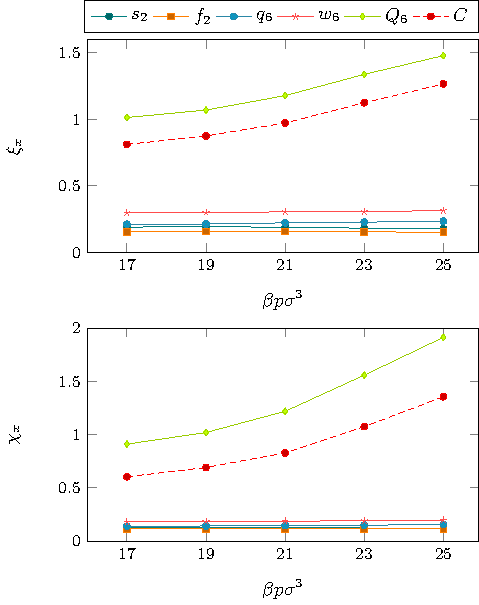
\includegraphics{fig_lengths}
	\caption{\textbf{Correlation length} extracted for two-body and many-body scalar order parameters, function of the pressure. Only many-body correlation lengths are increasing (only slightly for $\xi_{w_6}$), while the lenghscale associated with the two-body quantities is constant.}
	\label{fig:Fourierlengths}
\end{figure}

\begin{figure}
	\centering
	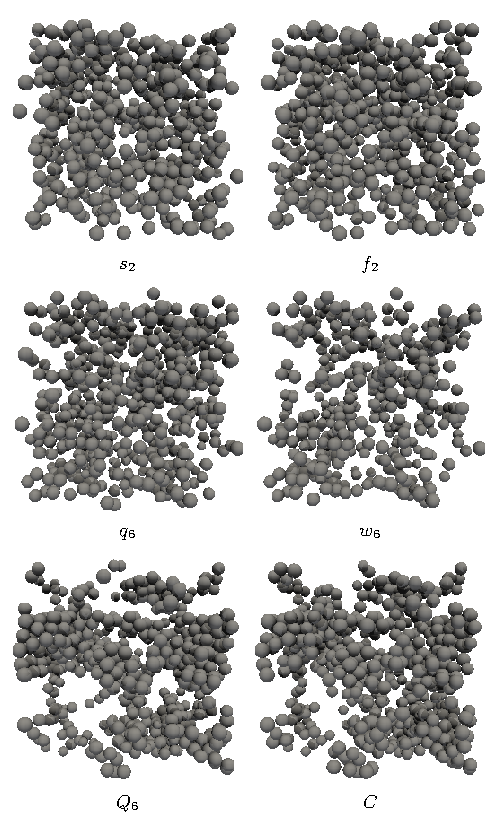
\includegraphics{fig_3D}
	\caption{\textbf{Visualisation of the ordered regions} defined by the various order parameters. All pictures correspond to a thin slice ($5\sigma$) of the same configuration at $\beta p\sigma^3=23$ and $\delta=7\%$. Only $Q_6$ and $C$ show meaningful fluctuations.}
	\label{fig:3D}
\end{figure}

The correlation lengths of crystal-like bond orientational order can be easily measured in real space due to the tensorial nature
of these order parameters, as was shown in previous studies~\cite{tanaka,kawasaki,mathieu_icosahedra,russo_gcm,russo_hs}. Two-body
correlation functions, being $f_2$ and $s_2$ both scalars, is more difficult to extract in real-space, especially at long distances,
where long averages are required to overcome the statistical noise. A more reliable procedure to extract correlation length can
be obtained by measuring correlation lengths in Fourier space.
The procedure is the following.
For any scalar order parameter field $x$ increasing with order, we define the threshold 
\begin{equation}
x^* \equiv \langle x\rangle + \sqrt{\langle x^2\rangle - \langle x\rangle^2},
\label{eq:xstar}
\end{equation}
at one standard deviation above the average value. We then compute a four-point structure factor keeping only the ordered particles ($x>x^*$). The thresholds are indicated on Fig.~\ref{fig:distrib}. Formally we define a function $\omega(i) = \Theta [x(i) - x^*]$, where $\Theta(x)$ is Heaviside’s step function, and a four-point structure factor
\begin{equation}
	S_x(q) = N^{-1}(\left\langle \Omega(\mathbf{q}) \Omega(-\mathbf{q}) \right\rangle - | \left\langle \Omega(\mathbf{q}) \right\rangle^2 |),   
	\label{eq:StrutureFactor}
\end{equation}
where $\Omega(\mathbf{q})$ is the Fourier transform of $\omega(i)$: 
\begin{equation}
	\Omega(\mathbf{q}) = \sum_i \omega(i)\exp(-\imath \mathbf{q}\cdot\mathbf{r}_i).  
\end{equation}
The case of order parameters decreasing toward ordering (i.e. $s_2$, $w_6$) is trivially obtained by changing the sign.

Fig.~\ref{fig:structurefactor} shows the small wave-vector increase of $S_x(q)$, which is well described by the asymptotic Ornstein-Zernike function in Fourier space:
\begin{equation}
	S_x(q\rightarrow 0) \approx \frac{\chi_x}{1+\xi_x^2 q^2},
	\label{eq:OZ_Fourier}
\end{equation}
where $\xi_x$ is the correlation length and $\chi_x$ the susceptibility. In general, an independent determination of $\chi_x$ is crucial for the fit~\cite{Flenner2011}. However here we deal with correlation lengths much smaller than the simulation box and both $\xi_x$ and $\chi_x$ can be reliably estimated from a two parameter fit of $S_x(q)$.

For overall coherency, we have used the above procedure not only for the two-body $s_2$ and $f_2$, but also for scalars derived from the multi-body bond orientational order, i.e. $q_6$, $w_6$, $Q_6$ and $C$. The dependence on the pressure of the resulting correlation lengths is shown on Fig.~\ref{fig:Fourierlengths}. Most of the order parameters produce constant lengthscales, including the two-body quantities and $q_6$, $w_6$ that are sensible to icosahedral order. The only growing lengths are extracted from measures of local crystal-like order, i.e. $Q_6$ and $C$. We confirm that the same results are obtained from real-space correlation functions. The absence of correlations for two-body quantities is suggested in the first row of Fig.~\ref{fig:3D}. Only $Q_6$ and $C$ (last row in Fig.~\ref{fig:3D}) show clustering of the ordered particles on medium range.

The length scales obtained from $Q_6$, $C$ in Fourier space or from the tensorial $\mathbf{q}_6$ or $\mathbf{Q}_6$ (not shown) are similar increase monotonically with pressure. Note that the scalar $q_6$ (dominated by the icosahedral order) yields a very different correlation length. We checked that the constancy of the length of two-body parameters was not affected by the definition of the threshold $x^*$, either smaller, larger or equal to the average value $\langle x\rangle$ (the absolute value of the length is marginally affected by this definition, but not the pressure dependence). Coherently, real-space correlation function (not shown) of $f_2$ (respectively $s_2$) are perfectly identical at all pressures.

The study of correlation lengths have shown that by increasing pressure, the range of
crystal-like bond-orientational order increases, and as shown in Ref.~\cite{tanaka,mathieu_icosahedra}
driving the slowing down of the system. Bond-orientational order corresponds to
orientationally ordered regions which spontaneously form in the metastable phase.
$f_2$ is instead decoupled from the relevant structures involved in the transition, as
was shown in Fig.~\ref{fig:f2decoupling}.


\subsection{Competition between icosahedral arrangements and crystalline arrangements}\label{sec:icosahedra}

\begin{figure}
 \centering
 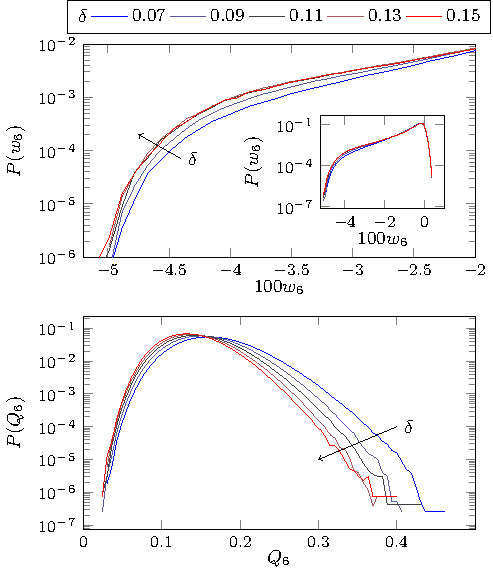
\includegraphics{fig_polydistrib}
 \caption{\textbf{Effect of polydispersity} on local structures at constant pressure ($\beta p\sigma^3=23$). \textbf{top} detail of the distribution of $w_6$ (full distribution in inset) showing a small increase in the icosahedra population saturating around $10\%$. \textbf{bottom} distribution of $Q_6$ showing a marked decrease in the crystallinity.}
 \label{fig:polydispersity}
\end{figure}

We will now focus on the state point at $\beta p\sigma^3=23$ at different polydispersities to
study the mechanism by which polydispersity disfavors the crystallization transition.

In Fig.~\ref{fig:polydispersity} we show the probability distributions for the order
parameters $Q_6$ and $w_6$ at different polydispersities. It is immediately
evident that, while bond-orientational order is rapidly suppressed with increasing
polydispersity (as shown in the suppressed signal at high $Q_6$), particles in icosahedral
environments are not disfavored by polydispersity. On the contrary the fraction of
icosahedral particles increases with polydispersity, and saturates at around $\delta=10\%$.

\begin{figure}
 \centering
 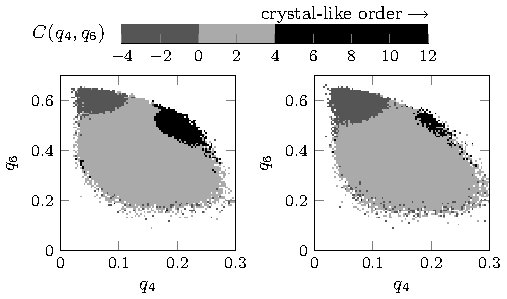
\includegraphics{fig_Cmaps}
 \caption{Average crystallinity order parameter projected in the $q_4$,$q_6$ space for the metastable fluid at $\beta p\sigma^3=23$ at $\delta=7\%$ (top) and $\delta=15\%$. Icosahedra appear in the top-left corner of each plot and perfect \textsc{fcc} crystals would be in the top-right corner.}
 \label{fig:Cmaps}
\end{figure}


Figure~\ref{fig:Cmaps} shows that the metastable fluid distribution presents both characteristic
structures: icosahedral environments with high $q_6$, low $q_4$ and negative $C$; crystal-like bond ordered regions with high values of
$q_4$, $q_6$ and $C$. The main difference between the low and
high polydispersity metastable states is the population of the crystal-like bond ordered regions.


\begin{figure}
 \centering
 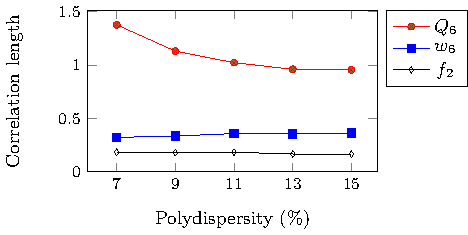
\includegraphics{fig_lengthpoly}
	\caption{\textbf{Polydispersity dependence of the correlation lengths} at $\beta p\sigma^3=23$. The dominant crystalline length decreases, the icosahedral length increases, however they plateau well before crossing. The two-body length shows no indication of becoming dominant with increasing $\delta$, even decreasing slightly.}
	\label{fig:lengthpoly}
\end{figure}

In the same way, the correlation length extracted from $Q_6$ decreases with increasing polydisersity, while the one extracted from $w_6$ increases (see Fig.~\ref{fig:lengthpoly}). However the two lengths are far from crossing and seem to saturate around $\delta=13-15\%$. The correlation length of $f_2$ is constant or even slightly decreasing with $\delta$, not at all taking over the many-body lengths. Thus, in the present range of polydispersity, crystal-like bond order fluctuations is still dominating the system static (and dynamic~\cite{mathieu_icosahedra}) properties.

In Ref.~\cite{russo_hs} we have shown that the competition between crystalline packings and
isosahedral packings can be studied via two-dimensional maps of translational vs orientational order.
Orientational order is captured by $q_6$, which is small for disordered arrangement of particles and
increases for both crystalline and icosahedral particles. Translational order is instead measured with
the local packing fraction, $\phi$, obtained by measuring the volume of the Voronoi diagram associated with
each particle. The calculation is straightforward: for each
configuration, crystalline particles are identified with the method described in Section~\ref{sec:methods} and the other particles are termed ``fluid''. For each subset of particles, the average value of the volume fraction $\phi$ is calculated as a function of the order parameter $q_6$, and plotted in Figure~\ref{fig:stability_map}.
For each value of $q_6$ the map captures the average volume fraction $\phi$ of both crystalline and non-crystalline
environments.

\begin{figure}
 \centering
 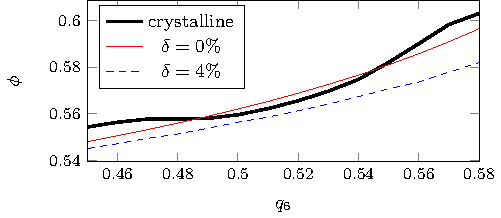
\includegraphics{fig_stability_map}
 \caption{Average $\phi$ as a function of $q_6$ for particles identified as fluid and crystalline. The continuous red curve represents fluid particles in a system at $\beta p\sigma^3=17$ and $\delta=0\%$, while dashed blue curve represents fluid particles at the same pressure but at $\delta=4\%$. The thick black curve represents instead solid particles (this curve is less sensitive to polydispersity and it is reported once).}
 \label{fig:stability_map}
\end{figure}
In Fig.~\ref{fig:stability_map}
we compare the curves at $\beta p\sigma^3=17$ and at different polydispersities:
at $0\%$ (monodisperse system, black circles) and at $4\%$ (red squares). The curve for the
crystalline particles is similar at the two considered polydispersities and is reported once
as the dashed line. First we consider the monodisperse case. As shown in the figure,
at low volume fraction, a particle in the fluid phase has higher orientational order than in the crystalline phase.
But at $\phi\cong 55.8\%$ a crossover
occurs and the crystal phase gains microscopic stability: a particle in a crystalline environment will
have higher orientational order than a particle in the fluid phase at the same volume fraction.
This crossover marks the appearance in the fluid phase of the metastable crystals which continously
appear, grow and shrink, until eventually a crystal droplet reaches the critical size and starts the
crystallization process.
At higher volume fractions ($\phi\cong 58\%$) another crossover occurs, with
crystalline particles having less orientational order than particles in the ``fluid'' branch.
These particles in the fluid phase at high $q_6$ are easily identified as particles in icosahedral packings (they have
a low value of $w_6$).
It is thus clear that icosahedral packings are competing with crystalline packings, eventually dominating
at high $\phi$. This scenario is confirmed by looking at the polydisperse case (red squares in
Figure~\ref{fig:stability_map}).
At polydispersity $\delta=4\%$ the crystalline branch always lays above the fluid one, meaning that
crystalline environments, at any fixed $\phi$, are not able to attain higher volume orientational order than other configurations.
Microscopically the difference between the monodisperse case and the polydisperse case, is due to an increased population of icosahedral particles, which dominate the fluid branch for $q_6\gtrsim 0.5$.
We have shown that, while for the monodisperse case there is a range of volume fractions where crystalline particles
attain higher orientational order than icosahedral arrangements, for the polydisperse case icosahedral
particles always attain higher orientational order.
This is immediately reflected in direct simulations,
as at this pressure it is not possible to crystallize simulations at $\delta=4\%$, while the
monodisperse simulations are easily crystallized.

We have thus provided direct evidence that icosahedral particles are responsible for the suppression
of crystallization in polydisperse hard spheres.

\section{Discussion}\label{sec:discussion}

In the present study we have compared the evolution of static length scales in polydisperse hard spheres
for both two-body and many-body correlation functions. While two body correlation functions do not
show any sign of an increasing length scale with pressure, we have confirmed that in the glass transition of polydisperse hard spheres the relevant static length is the correlation length of the crystalline bond order.
We have also determined the relevant microscopic structures that are associated with the increasing
lengthscale: they correspond to crystalline environments of particles and are characterized by slow
dynamics.
We thus confirm that in the glass transition of polydisperse hard spheres the relevant static length is the correlation length of the crystal-like bond orientational order.

The other relevant structure with slow dynamics are icosahedral packings of particles, but
their lenghscale doesn't grow appreciably with increasing pressure. Icosahedral assemblies of particles
are spatially uncorrelated. While not having a direct role in the slowing down of the dynamics, we
have shown that icosahedral packings are responsible for the avoidance of the crystallization transition
with increasing polydispersity.
The increase in polydispersity reduces the degree of crystal-like bond orientational order whereas enhances the icosahedral order (see Fig. \ref{fig:Cmaps}). 
The former is crucial for triggering 
crystal nucleation \cite{russo_hs}, the latter leads to the frustration against crystallization, a role that increases with polydispersity. None of these physical aspects of the system could be described by two-body quantities. 

We previously showed that spatial fluctuations of crystal-like bond orientational order are closely correlated with local dynamics: 
more ordered regions have slower dynamics \cite{KAT,WT,ShintaniNP,tanaka,Kawasaki3D,mathieu_icosahedra}. 
Together with these results, we may say that it is many-body correlations, or crystal-like bond orientational ordering, that 
are the cause of slow dynamics and dynamic heterogeneity.  
This means that future theories of glass transition should deal with many-body correlation effects properly. 
The link between the symmetry of the relevant bond order parameter for describing structural ordering 
in a supercooled liquid and that for crystallization is another interesting point. 
This may be a direct consequence of the fact that glass transition is governed by the same free energy as that 
describing crystallization. This conjecture is further supported by our second finding on the mechanisms by which 
polydispersity increases the glass-forming ability of hard spheres.  

The mechanism by which polydispersity increases the barrier for crystal nucleation may be two fold: 
(i) direct random disorder effect which destroys crystal-like bond orientational order in a supercooled liquid,
which is the first step in crystal nucleation~\cite{russo_hs};
(ii) enhancement of icosahedral ordering with an increase in the polydispersity.
It is known that size disparity between a particle and its surrounding neighbours stabilizes icosahedral order \cite{Shimono2012}. 
Since the symmetry of icosahedral order is not consistent with that of the equilibrium crystal polymorphs (fcc and hcp for this case), 
competing ordering toward these two mutually inconsistent symmetries leads to strong frustration effects on crystallization, as in the case of 
2D spin liquids~\cite{ShintaniNP,STNM}. 

Although we studied polydisperse hard spheres in this article, these mechanisms should be relevant to many other 
glass-forming systems including metallic glass formers~\cite{Jakse2008,Hwang2012}. 

\section{Summary}


In this article, we show firm evidence for the importance of many-body correlations in glass transition phenomena 
for hard spheres liquids. This feature cannot be described by the standard liquid-state theories based on two-body correlation. 
This implies that, at high density, liquid state packing effects inevitably lead to many-body correlations, which play 
key roles in phenomena like the glass transition and crystallization. 
A physically natural order parameter to pick up these many-body correlations is \emph{bond order parameter}, whose importance 
has been well recognized and established for ordering transitions of hard disks in 2D \cite{NelsonB}. 
We believe the importance of incorporation many body correlations into theories to describe
both the glass transition and crystallization phenomena properly~\cite{TanakaJSP,TanakaR}.

Our study also indicates that there is an intrinsic link between crystallization and vitrification. 
Whether a polydisperse hard spheres system is crystallized or vitrified can be controlled just by changing 
polydispersity, which affects extendable crystal-like bond orientational order and isolated icosahedral order 
in an opposite manner.
We speculate that this direct link may exist for systems where crystallization does not involve phase separation, 
in other words, as far as the two phenomena are described by the same free energy \cite{TanakaGJPCM,TanakaJSP,TanakaR}.  
How universal is this scenario needs to be checked carefully in the future. 

\section*{Acknowledgements}
This study was partly supported by a grant-in-aid from 
the Ministry of Education, Culture, Sports, Science and Technology, Japan (Kakenhi)
and by the Japan Society for the Promotion of
Science (JSPS) through its ``Funding Program for World-Leading
Innovative R\&D on Science and Technology (FIRST Program)'' and a JSPS Postdoctoral Fellowship.


%\paragraph*{\bf Author Contributions}
%M.L., J.R. and H.T. conceived the research, discussed and wrote the manuscript ; J.R. performed the simulations, M.L. and J.R. performed the analysis. M.L. and J.R. contributed %equally to this work.


\bibliographystyle{apsrev4-1}
\bibliography{biblio}

\end{document}
